\title{Computing PageRank}
\subtitle{\SubTitleName}
\institute[]{\Course}
\author{\Instructor}
\maketitle   


\frame{\frametitle{Topics and Objectives}
\Emph{Topics} \\
%\TopicStatement
\begin{itemize}

    % \item review of Markov chains

    % \item theorems describing the steady state of a Markov chain
    
    % \item applying Markov chains to model web traffic
    
    \item adjustments to the PageRank algorithm 
    
    \item calculating the PageRank of a web

\end{itemize}

\vspace{0.5cm}

\Emph{Learning Objectives}\\

%\LearningObjectiveStatement

\begin{itemize}

    % \item determine whether a stochastic matrix is regular
    
    % \item calculate the steady-state of a Markov process
    
    % \item apply matrix powers and theorems to characterize the long-term behaviour of a Markov chain

    \item construct a transition matrix and a Markov Chain for a given web to model web traffic and compute the PageRank of the web

\end{itemize}

\vspace{0.25cm} 

% \Emph{Motivating Question}

} 





\begin{frame}
\frametitle{Adjustments Needed}

Our mathematical model for PageRank (PR) has two problems.
\begin{itemize}
    \item the transition matrix is not regular: we do not have a unique steady-state
    \item pages that do not link to other pages can have the largest importance, or highest PageRank
\end{itemize}

\end{frame}


\begin{frame}
\frametitle{Adjustment 1}

    
    \begin{center}\begin{tikzpicture} \node [mybox](box){\begin{minipage}{0.85\textwidth}
        \vspace{4pt} 
        If a user reaches a page that does not link to other pages, the user will choose any page in the web, with equal probability, and move to that page.
    \end{minipage}};
    \node[fancytitle, right=10pt] at (box.north west) {Adjustment 1};
    \end{tikzpicture}\end{center}


    \vspace{6pt} 
    
    We will denote this modified transition matrix as $P_*$. 

\end{frame}


\begin{frame}\frametitle{Adjustment 1 Example}

    \begin{center}
        \begin{tikzpicture}
            \begin{scope}[->,>=stealth',shorten >=0pt,auto,node distance=1.5cm,very thick, main node/.style={circle,fill=black!05,draw}]
            \node[main node] (1) {A};
            \node[main node] (2) [right of=1] {B};
            \node[main node] (3) [below of=1] {C};
            \node[main node] (4) [below of=2] {D};
            \node[main node] (5) [right of=4] {E};
            \path[every node/.style={font=\sffamily\small}]
            (1) edge node[below] {} (2)
            (1) edge node[below] {} (4)
            (2) edge node [above] {} (3) 
            (3) edge node {} (1)
            (4) edge node [above] {} (5);
            \end{scope}
        \end{tikzpicture}  
    \end{center}    
    
    $P$, and $P_*$ are as follows.
    
    \pause
    
    $$P = \spalignmat{0 0 1 0 0;.5 0 0 0 0;0 1 0 0 0;.5 0 0 0 0;0 0 0 1 1}, \quad P_* = \spalignmat{0 0 1 0 .2;.5 0 0 0 .2;0 1 0 0 .2;.5 0 0 0 .2;0 0 0 1 .2}$$
    

\end{frame}



\begin{frame}
\frametitle{Adjustment 2}

    \begin{center}\begin{tikzpicture} \node [mybox](box){\begin{minipage}{0.85\textwidth}
        \vspace{4pt} 
        A user at any page will navigate to any page among those that their page links to with equal probability $p$, and to any page in the web with equal probability $1-p$. The transition matrix becomes $$G = pP_* + (1 - p)K.$$
        All the elements of the $n\times n$ matrix $K$ are equal to $1/n$. 
    \end{minipage}};
    \node[fancytitle, right=10pt] at (box.north west) {Adjustment 2};
    \end{tikzpicture}\end{center}

    \vspace{6pt} 
    
    Note the following.
    \begin{itemize}
        \item  $p$ is referred to as the \Emph{damping factor}, Google is said to use $p = 0.85$. % \\[12pt] With adjustments 1 and 2, our the Google matrix is:
        \item Adjustment 2 forces $G$ to be regular stochastic when $0\le p < 1$.
    \end{itemize}
    
   
    
    
    
\end{frame}



\begin{frame}\frametitle{Google Matrix Example}


    \begin{center}
        \begin{tikzpicture}
            \begin{scope}[->,>=stealth',shorten >=0pt,auto,node distance=1.5cm,very thick, main node/.style={circle,fill=black!05,draw}]
            \node[main node] (1) {A};
            \node[main node] (2) [right of=1] {B};
            \node[main node] (3) [below of=1] {C};
            \node[main node] (4) [below of=2] {D};
            \node[main node] (5) [right of=4] {E};
            \path[every node/.style={font=\sffamily\small}]
            (1) edge node[below] {} (2)
            (1) edge node[below] {} (4)
            (2) edge node [above] {} (3) 
            (3) edge node {} (1)
            (4) edge node [above] {} (5);
            \end{scope}
        \end{tikzpicture}  
    \end{center}    
    
    The Google matrix for this web, with $p = 0.85$ is $G = 0.85P_* + 0.15K$, where
    
    \pause
    
    $$P_* = \spalignmat{0 0 1 0 .2;.5 0 0 0 .2;0 1 0 0 .2;.5 0 0 0 .2;0 0 0 1 .2}, \quad K = \frac 15 \spalignmat{1 1 1 1 1;1 1 1 1 1;1 1 1 1 1;1 1 1 1 1;1 1 1 1 1;}$$

\end{frame}



\begin{frame}

\frametitle{Computing Page Rank}

\begin{itemize}
	\item Because $G$ is regular stochastic, for any initial probability vector $\vec x_0$, $$\lim_{n \rightarrow \infty} G^n \vec x_0 = \vec q.$$ \pause

	\item We can obtain steady-state evaluating $G^n\vec x_0$ for large $n$, by solving $G\vec q = \vec q$, or by evaluating $\vec x_n = G \vec x_{n-1}$ for large $n$.\pause
	\item Elements of the steady-state vector give the importance of each page in the web, which can be used to determine PageRank. \pause
	\item Largest element in steady-state vector corresponds to page with PageRank 1, second largest with PageRank 2, and so on.

\end{itemize}


\end{frame}

\begin{frame}
\frametitle{Computing Page Rank: Exams}

On exams,
\begin{itemize} 
	\item problems that require a calculator will not be on exams
	\item if asked to construct $G$ for a given web, you can leave your answer as a sum of two matrices
\end{itemize}
    
\end{frame}



\begin{frame}[fragile=singleslide]
\frametitle{WolframAlpha and MATLAB/Octave Syntax}

    You will need to compute matrix powers in course activities and possibly in future courses.
    
    \vspace{12pt}
    
    Suppose we want to compute $
        \spalignmat{.8 .1 .2; .2 .6 .3; .0 .3 .5}^{10} .$
    
    \begin{itemize}
        \item At wolframalpha.com, we can use the syntax:
    {\small 
    \noindent \begin{verbatim}MatrixPower[{{.8,.1,.2},{.2,.6,.3},{.0,.3,.5}},10]\end{verbatim}}
    
        \item In MATLAB, we can use the syntax
    {\small 
    \noindent \begin{verbatim}[.8 .1 .2 ;.2 .6 .3;.0 .3 .5]^10\end{verbatim}}    
        \item Octave uses the same syntax as MATLAB, and there are several free, online, Octave compilers. For example: https://octave-online.net. 
    \end{itemize}

\end{frame}





\begin{frame}
\frametitle{PageRank Early History}


\begin{itemize}
    \item  When PageRank was devised, in 1996, Yahoo! used humans to provide an ``index for the Internet" which was 10 million pages at the time.
    \item  The PageRank algorithm was produced as a competing method.  The patent was awarded to Stanford University, and exclusively licensed to the newly formed Google corporation. 
    \item Brin and Page combined the PageRank algorithm with a webcrawler to provide regular updates to the transition matrix for the web.  
\end{itemize}



\end{frame}



\begin{frame}
\frametitle{There is (of course) Much More to PageRank}

\begin{columns}
\begin{column}{.55\textwidth}

\begin{itemize}
    \item The explosive growth of the web soon overwhelmed human based approaches to searching the Internet. 
    \item The PageRank Algorithm currently used by Google is under constant development, and tailored to individual users. 
\end{itemize}

\end{column}\begin{column}{.4\textwidth}
\begin{center}
        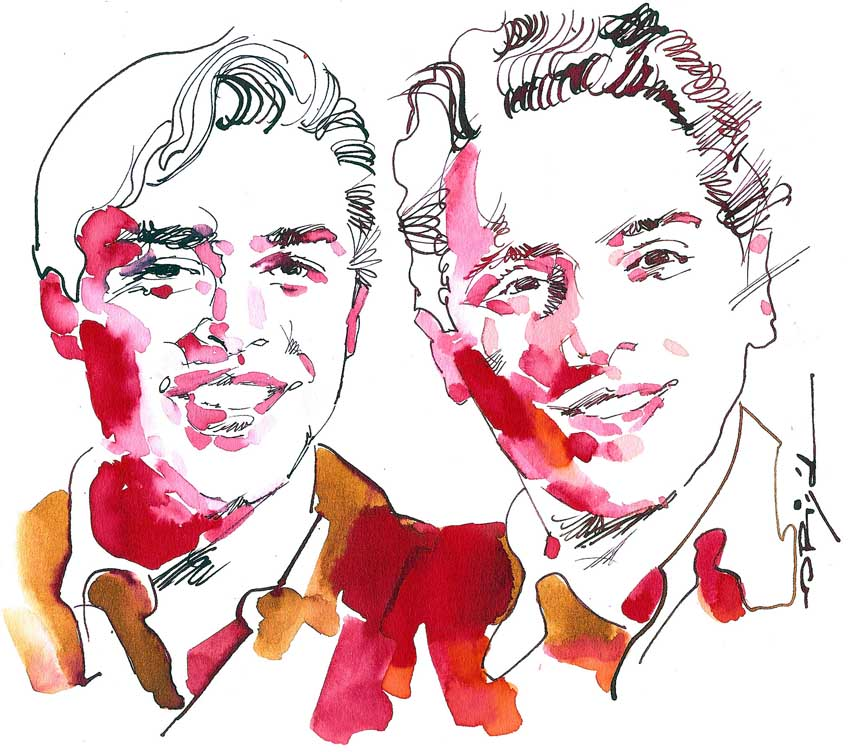
\includegraphics[width=1.0\textwidth]{Chapter5/images/PageBrin.jpg} 
        \begin{center}
        \vspace{-8pt}
    {\tiny
    \textit{image by Graziano Origa, copyright CC BY-SA 3.0}
    }
    \end{center}
\end{center}


\end{column}
\end{columns}
    

\end{frame}


\frame{\frametitle{Summary}

    \SummaryLine \vspace{4pt}
    \begin{itemize}\setlength{\itemsep}{8pt}

    \item constructing a transition matrix and a Markov Chain for a given web to model web traffic and compute the PageRank of the web
    
    \item numerical approaches to computing PageRank
    
    \end{itemize}
    
    \vspace{8pt}
    \pause 
}


% \begin{frame}
% \frametitle{Example 2 (if time permits)}



%     Construct the Google Matrix for the web below. Which page do you think will have the highest PageRank? How would your result depend on the damping factor $p$? Use software to explore these questions.     
%         \begin{center}
%         \begin{tikzpicture}
%             \begin{scope}[->,>=stealth',shorten >=1pt,auto,node distance=1.5cm,thick, main node/.style={circle,fill=black!05,draw}]
%             \node[main node] (1) {A};
%             \node[main node] (2) [right of=1] {B};
%             \node[main node] (3) [below of=1] {C};
%             \node[main node] (4) [below of=2] {D};
%             \path[every node/.style={font=\sffamily\small}]
%             (1) edge node [above] {} (3)
%             (3) edge node [above] {} (4)
%             (2) edge node [above] {} (3);
%             \end{scope}
%         \end{tikzpicture}  
%     \end{center}    

% \end{frame}

